\section{Needfinding}
\label{sec:needfinding}

Need finding was already mostly completed during last quarter. For this quarter, we found out more about Audi owners and visited a truly smart home and talked with its owner.

\subsection{More on Audi Owners}

Upon interviewing additional users this quarter, a key driver for Audi owners became apparent: understated elegance. One well-off Audi owner, who has had 9 or 10 Audis in his lifetime, buys them because they are well-designed, practical (e.g. 4WD standard), and not as pretentious as BMW. This sentiment is mirrored in the Audi TV spot "Performance with the Right Attitude"~\cite{AudiTVSpotAttitude}. Audi owners love the experience of driving an Audi, and even with the recent emissions scandal, one Audi owner said that the Facebook ads to join class action lawsuits against VW were met with comment after comment in defense of the Audi brand and experience. One woman said that she will never buy another car, because she is not sure if she'll be able to buy another Audi diesel, and loves it so much she would never want to get rid of it. While Audi matches the performance of many other luxury cars, it does not accompany performance with cache or arrogance, and that image is appealing to many owners.

Not many Audi owners we interviewed were interested in the technological aspects of the car, let alone the smart home. Though one user did say he bought an A7 because it was the most technologically advanced at the time, but considers himself "technologically compromised" and does not use as many of the features as he expected. He finds the Audi interface a bit confusing, and the setup cumbersome, as did several other luxury car owners we spoke with.

\todo{\{Jonathan\}My hunch is that this use case is too niche and the we should leave this part out}
One unique use case that arose out of these interviews was the case of second home ownership. If someone is fortunate to own a second home and divide their time between two homes, there are unique needs that could be addressed. For instance, one couple lives in 2 homes and owns a total of 3 cars, and has to carry around different keys for each at any given time. If there was a unique system that allowed them to carry around a single key fob for all homes and cars, they would be very interested in that. However, that also brought up the security issue if someone did lose a key fob, it could be used to get into some of the most valuable aspects of their lives, so there would need to be ample safeguards for that. Also, one would still need basic keys for valet parking, housekeepers, etc. There is potential in unifying home and car keys for multiple cars and homes into one incredibly secure device, perhaps as an addition to the smart phone, that can be easily tracked and disabled if misplaced or stolen, due to its importance and value.

\subsection{Visiting a True Smart Home}

One user that we visited, Jack, owns a home that is wired with Control 4 lighting and media throughout the home. This allows Jack to preset certain actions on the switches, such as briefly turning on a series of lights for his daughter to get to her room at night. He has over 20 different events that are programmed. However, we found that he is the only person in his family who is familiar with the system and is comfortable using it.

Jack also owns a home security system, but seldom uses it, as he only has 20 seconds to disarm it upon arrival at home, and the false positives, as mentioned above, are more trouble than it's worth. However such a system does lower his insurance premium, which is a primary reason to keep it. That and on vacations, they can know that the house is secured.

\todo{\{Jonathan\} I don't think this is about the interface. 20 seconds is just too short.}
This visit uncovered the need for more streamlined interface with a homeowner's security system. Similar sentiments have been echoed by other user interviews as well. At the same time, this visit confirmed our earlier suspicions about the complexity of smart home setup and use.

\section{From Needs to Prototypes} %Once the development of prototypes is done, this section could be interwoven with that material.

In designing a system for Audi owners, we must keep in mind that it must be simple, easy to set up (or include setup with purchase) and not too much add additional complexity. From both our interviews and consumer surveys on smart homes, it is apparent that innovation for the sake of innovation is a necessary but not sufficient condition for smart home technology adoption, and our system should not just be another gizmo that can be patched into existing systems. It therefore has to address an underlying problem, anxiety, or need of Audi users.

The basis for every prototype we built and will build are the needs of our actual users. In order to find out about these needs we conducted a series of interviews with potential users and used our findings and insights from testing prototypes to iterate those needs or even discover new needs. This section will give an overview over the needs we identified when it comes to the car, the house or the transition between both.The set of needs we focused on for our resulting problem statement will be presented as well.

We interviewed a great variety of potential users, including Audi owners, families and smart home users and identified multiple basic needs when it comes to using technology in general as well as smart home technology in particular. One of them is simplicity: Users reported that they connect current smart home technologies with cumbersome setup processes and a lack of standards. Instead, they want them to be easy to setup, to integrate seamlessly into their existing technological ecosystem and to function reliably. Similarly, some report that they feel current car technology is too complex for them, resulting in many users not making use of their many in-car features. They demand a more user-friendly interface. This includes multiple users explicitly stating that they prefer a physical interface like buttons over "just another app".

Security is a great concern of many users. Especially when it comes to smart home technology, many were worried about the fact that their house has a lot of dense and very private information about them. Moreover, many feared that a smart home would be vulnerable to attacks. Their requirement for any system being part of a smart home would thus be absolute data security and also privacy. On the other hand, many can imagine to use smart home technology to make their house more secure while they are gone, monitoring things such as the entrance door or windows. 

Especially when it comes to the car but also when asked about the transition from car to house and vice versa, people value a certain comfort and convenience factor and enjoy entertainment. Especially Audi drivers even expect a certain level of comfort - their car is often a status symbol for them and as such it has to be well-manufactured, using only the best materials. 

Another need people often verbalized was freedom and flexibility. They valued the freedom that owning a car gave them such as being able to get anywhere at any time without being bound to things like the public transport schedule or having to book tickets many weeks in advance. In their car they are free to do whatever they want to unlike in most other spaces nowadays - whether it is listening to loud music, singing or sleeping. Their car also allows them to be more flexible, for example when it comes to heavy or bulky baggage such as sports equipment which would not be easily transportable with public transportation without prior planning. In consequence, one important need when it comes to smart homes would be for many that it the technology used is flexible and adapts to their routines without them needing to adjust settings themselves every time they deviate from their normal daily routine. 

While users do want their technologies to be smart to a certain level and adapt to their behavior automatically to ensure flexibility, they also want to maintain some level of control. This also applies to areas like autonomous vehicles where Audi drivers in particular reported that they actually really enjoy the act of driving and would not even want to own an autonomous car since it takes away too much of their control. 

By incorporating these basic needs into multiple prototypes we were able to identify more specific needs when it comes to the transition between the home and the car and vice versa. One major pain users had was carrying heavy things from their car into their house. The biggest use case here was the weekly grocery shopping that can become very heavy very fast especially with families. But also other daily or onetime activities that include carrying heavy things from the car to the house or the other way around such as garden work or vacations were mentioned as pain points that hamper the car-home-transition.

Another pain point we found for both, daily as well as exceptional or onetime activities, is that there is a loss of information in the transition space of home and car. This loss of information can roughly take on three different forms: Information about the home, information about the car and information about things you need to pack and carry between the car and the home. Many people we interviewed tend to forget certain things when they leave the house, among which are their smart phone, their keys or things like sports clothes (see also Figure \ref{fig:testerathome}). Furthermore, many users want to know about their home's current status right before or after leaving the house. Examples here are information about whether all of the windows are closed or whether the heater and all of the lights are turned off. The counterpart is information about the car that they want to know about just after returning home or while they are at home. Such things could be knowing whether the car is safe and locked correctly, knowledge about the car's current maintenance status or gas level or whether the windows are icy and maybe need cleaning before the car can be used. All of this information or rather the lack of this information can hamper the transition or the connection between car and home. More details on the prototypes these needs stem from can be found in the appendix (cf. appendix \ref{sec:PreviousPrototypes}). 

\begin{figure}[ht]
\todo{This just sounds wrong}
\centering
	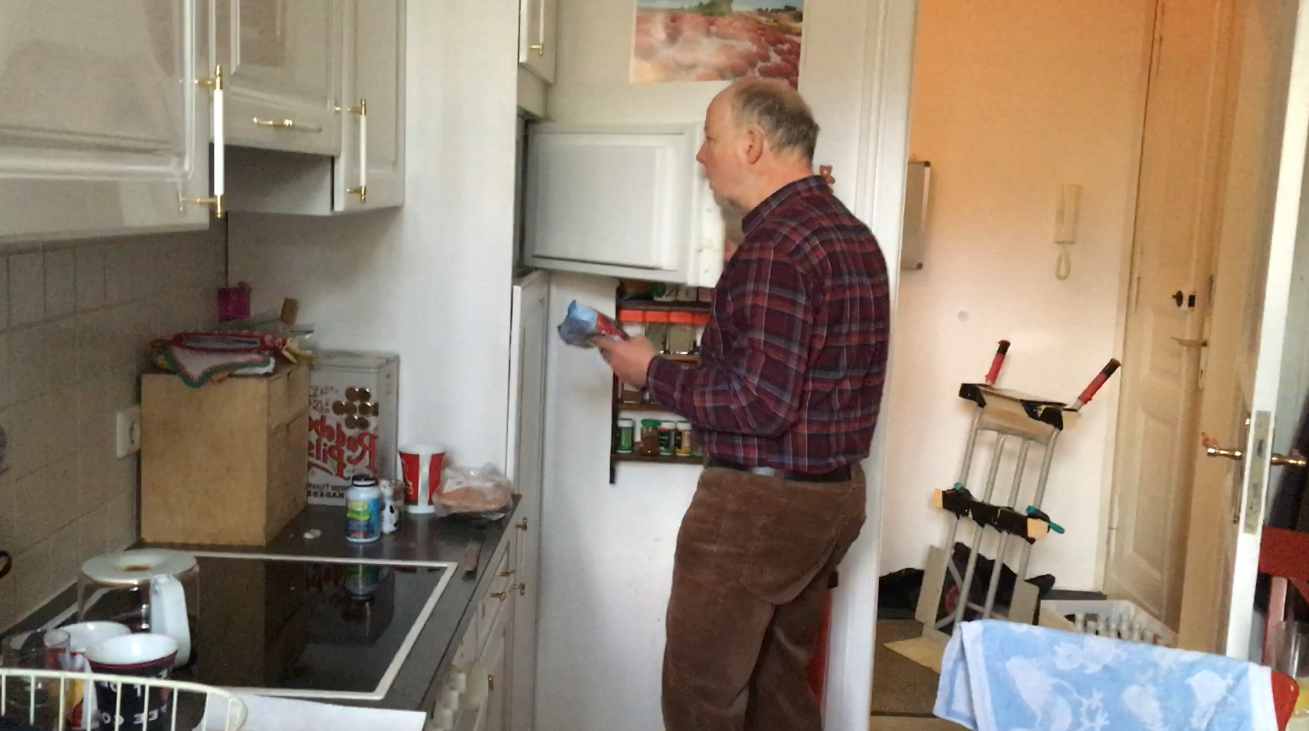
\includegraphics[keepaspectratio, width=\textwidth]{Figures/Needfinding/TesterAtHome}
	\caption{Tester checking whether everything is there}
	\label{fig:testerathome}
\end{figure}


